\documentclass[11pt]{article}

\usepackage[margin=1in]{geometry}
\usepackage{parskip}
\usepackage{hyperref}
\usepackage{lmodern}
\usepackage{graphicx}

\setlength{\parindent}{0pt}

\newcommand{\pullquote}[1]{
\vspace{0.5em}
\begin{center}
\textit{#1}
\end{center}
\vspace{0.5em}
}

\begin{document}

{\LARGE \textbf{Performance Scales More Easily Than Insight}}

\vspace{0.3em}

{\large Scaling and its limits in computational cognitive science}

\vspace{1em}

\textbf{Author:} Hanbo Xie -- Georgia Institute of Technology

\vspace{1.5em}

% ===== Lead Paragraph =====

\begin{center}
\begin{minipage}{0.9\textwidth}
\small
\textit{
In recent years, cognitive science has entered a new era of scaling. Large behavioral datasets, powerful AI models, and automated modeling pipelines now allow researchers to predict human behavior with unprecedented accuracy. Yet improved prediction does not automatically produce understanding. As performance scales rapidly, scientific insight often grows much more slowly. This essay argues that the emerging gap reflects two structural bottlenecks — in the data we collect and in how scientific knowledge itself is produced.
}
\end{minipage}
\end{center}

\vspace{2em}

% =====================

\section*{Opening}

As AI becomes increasingly influential in cognitive science, attitudes toward the integration of AI and psychology have become polarized. Some researchers believe AI will accelerate scientific discovery and perhaps even lead to unified theories of cognition. Others argue that AI contributes little to genuine scientific insight.

In the AI community, Rich Sutton’s essay \textit{The Bitter Lesson} argues that progress in artificial intelligence largely comes from scaling computation and data rather than relying on human-designed inductive biases.

This lesson is largely correct for engineering intelligent systems. But science is not only about building intelligence — it is about understanding it. Scientific progress ultimately depends on a particular kind of knowledge: insights that can be interpreted, communicated, and reused by others.

When the goal is to understand intelligence rather than simply build it, the relationship between scaling and progress looks different.

\pullquote{Performance scales more easily than insight.}

\begin{figure}[h]
    \centering
    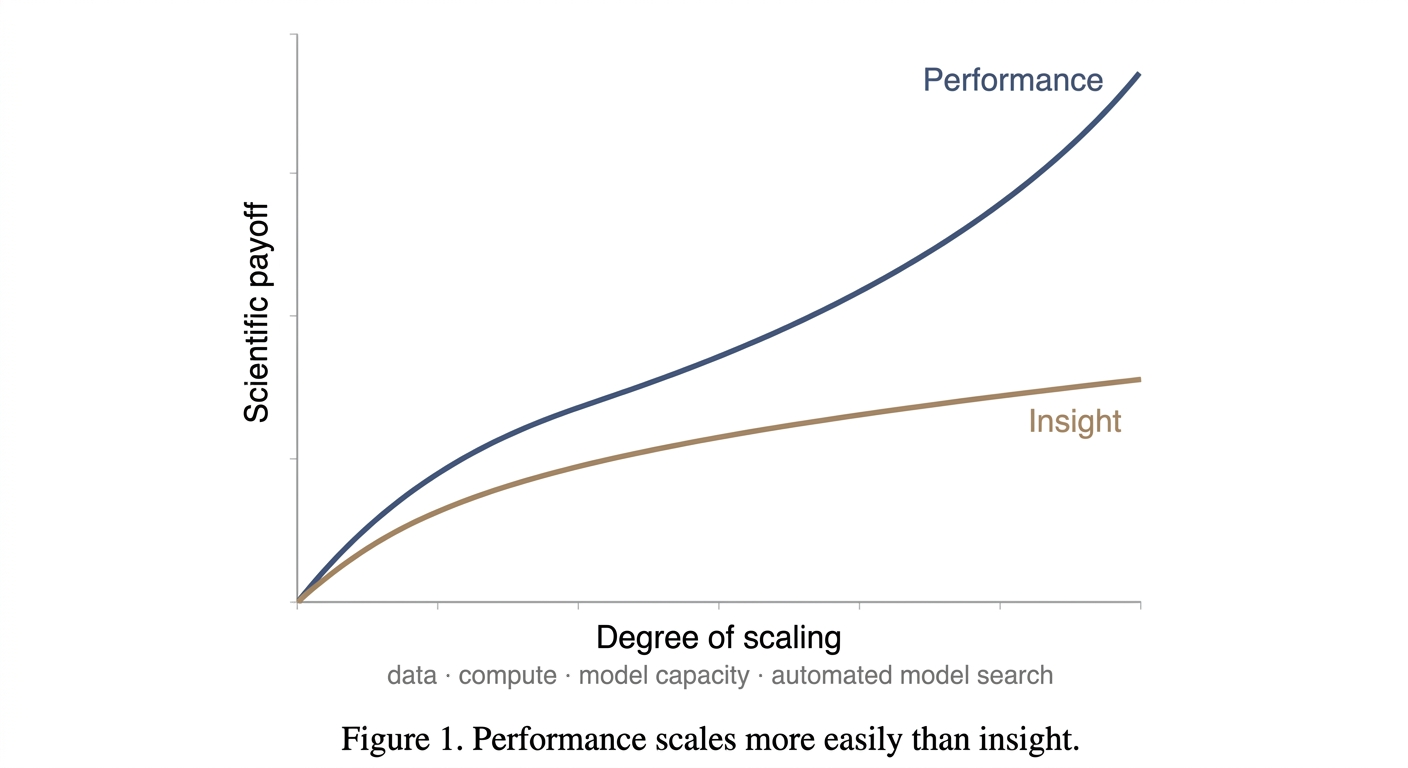
\includegraphics[width=0.88\textwidth]{figure1_performance_vs_insight.png}
    \label{fig:performance-insight}
\end{figure}

% =====================

\section*{Scaling Has Arrived}

Scaling has already arrived in cognitive science. Over the past decade, researchers have collected increasingly large behavioral datasets, sometimes involving tens of thousands of participants and millions of decisions. These datasets have enabled systematic comparisons between cognitive models and significantly improved our ability to predict human behavior.

At the same time, advances in AI have introduced new modeling paradigms. Neural networks and large language models can now be trained directly on behavioral datasets and often outperform traditional cognitive models in predictive accuracy. More recently, researchers have begun using AI systems to search for cognitive models, propose hypotheses, and even automate parts of the scientific workflow.

Together, these developments mark a methodological shift: cognitive science can now scale both data and models.

Yet a recurring pattern appears. Predictive performance improves rapidly, while scientific understanding grows much more slowly. Models may capture behavioral regularities, but they rarely tell us clearly what mechanisms they have learned or what new principles they reveal.

This gap reveals a deeper limitation of the current scaling paradigm.

% =====================

\section*{Bottleneck 1: Data}

\pullquote{We have scaled dataset size, but not the dimensionality of information they contain.}

Many large behavioral datasets are still collected within tightly controlled laboratory paradigms. These experiments are typically designed to isolate specific cognitive variables while minimizing noise.

While this strategy is valuable for hypothesis testing, it also limits the diversity of behaviors that can be observed. As a result, many datasets scale the number of participants or trials without substantially expanding the information contained in each observation.

A deeper problem arises from the nature of behavior itself. Observable choices are typically low-dimensional, while the cognitive processes generating them may be far more complex. As a result, many different mechanisms can produce the same behavior.

Without richer data, this many-to-one mapping makes it difficult to identify underlying cognitive processes.

One promising direction is to expand the dimensionality of measurement. In addition to behavioral choices, process-level signals such as verbal reports, eye movements, mouse trajectories, or planning traces may provide additional constraints on cognitive mechanisms.

The goal is not to replace behavioral data, but to complement it with richer observations that capture different aspects of cognition.

% =====================

\section*{Bottleneck 2: Knowledge}

\pullquote{We can search for models faster than we can understand them.}

A second bottleneck concerns how scientific knowledge is produced.

Modern AI systems can train complex models on behavioral datasets, search through vast spaces of candidate models, and generate hypotheses at unprecedented scale. These capabilities dramatically expand the search space of scientific models.

However, the ability to generate models does not automatically produce scientific insight.

Many discovered models lack clear semantic meaning. They may involve complex mathematical operations or high-dimensional representations that do not correspond to interpretable cognitive concepts.

Even when models achieve impressive predictive accuracy, it is often unclear what new principles of cognition they reveal. In many cases, the discovered mechanisms simply recombine existing ideas rather than introduce fundamentally new ones.

In other words, the production of models is scaling rapidly, but the production of insight is not.

This creates a growing asymmetry: we can explore model spaces faster than we can translate those models into scientific understanding.

\begin{figure}[h]
    \centering
    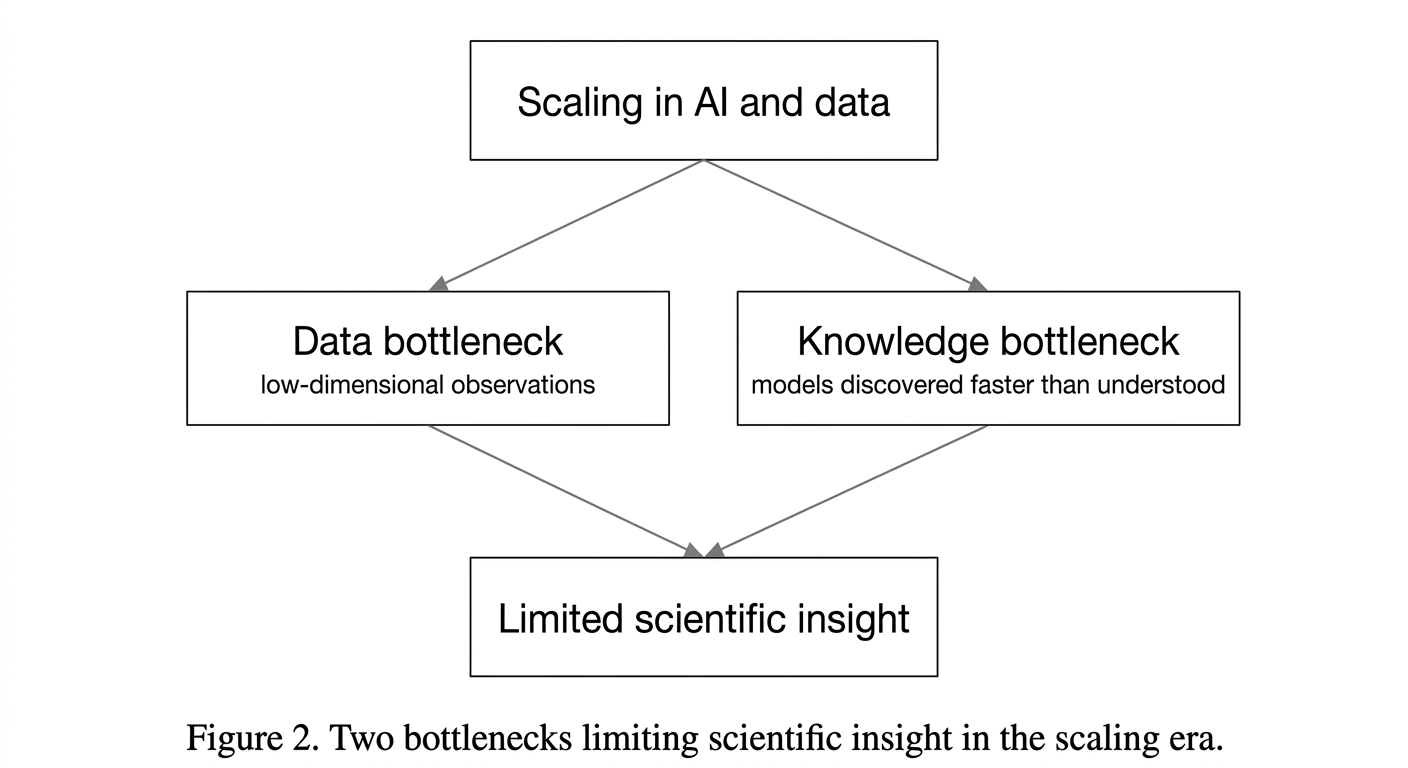
\includegraphics[width=0.85\textwidth]{figure2_two_bottlenecks.png}
    \label{fig:two-bottlenecks}
\end{figure}

% =====================

\section*{Interaction}

These two bottlenecks reinforce each other.

When datasets contain limited information about cognitive processes, model search is unlikely to uncover genuinely new mechanisms. Conversely, without strong conceptual frameworks, it becomes difficult to design experiments that generate more informative data.

As a result, scaling data and scaling models may yield diminishing returns for scientific understanding.

Addressing this problem may require new forms of collaboration between humans and AI systems, where modeling and conceptual interpretation develop together.

% =====================

\section*{Closing}

\pullquote{The question is not whether to scale, but what dimensions of science we should scale.}

Scaling will remain a central force in the age of AI. However, improving predictive performance alone does not guarantee deeper understanding.

Two directions may become increasingly important. First, cognitive science may need to expand the dimensionality of the data it collects, incorporating richer process-level measurements alongside behavioral outcomes.

Second, we may need clearer frameworks for evaluating scientific knowledge itself.

A scientific insight is not merely a model that predicts well. It is a form of knowledge that can be understood, communicated, and reused by other researchers.

Scientific knowledge matters precisely because it is transmissible. When a discovery can be expressed in a form that others can interpret, test, and build upon, it becomes part of our collective understanding.

Advancing cognitive science in the age of AI may therefore require not only stronger models and larger datasets, but also better ways of transforming model discoveries into shared scientific insight.

\end{document}